\subsection{Application client}
Le client developpé est une application Android. Nous avons choisi d'utiliser le langage Kotlin qui est plus performant et optimise les opérations et la structure par rapport à Java. C'est également le langage que nous utilisons au sein du cours d'Android, c'est donc un bon moyen de mettre en relation les deux cours.
Le rôle principal de ce client est de détecter (grâce au bluetooth) le Beacon le plus proche. En fonction de ce Beacon, le serveur Flask \acrshort{rest} est interrogé pour déterminer (via la base de données) dans quelle salle se trouve la personne et les \textit{\textit{devices}} présents (stores, radiateurs, lumières, etc.). Une fois l'emplacement déterminé et les \textit{\textit{devices}} détectés, les contrôles et les informations des différents \textit{\textit{devices}} apparaissent sur l'interface graphique de l'utilisateur, lui permettant de contrôler ou obtenir les différentes informations actuelles des \textit{\textit{devices}} et passées (sur les trois dernières heures) à proximité. La figure \ref{app_android} illustre le résultat obtenu.
\begin{figure}
    \begin{center}
        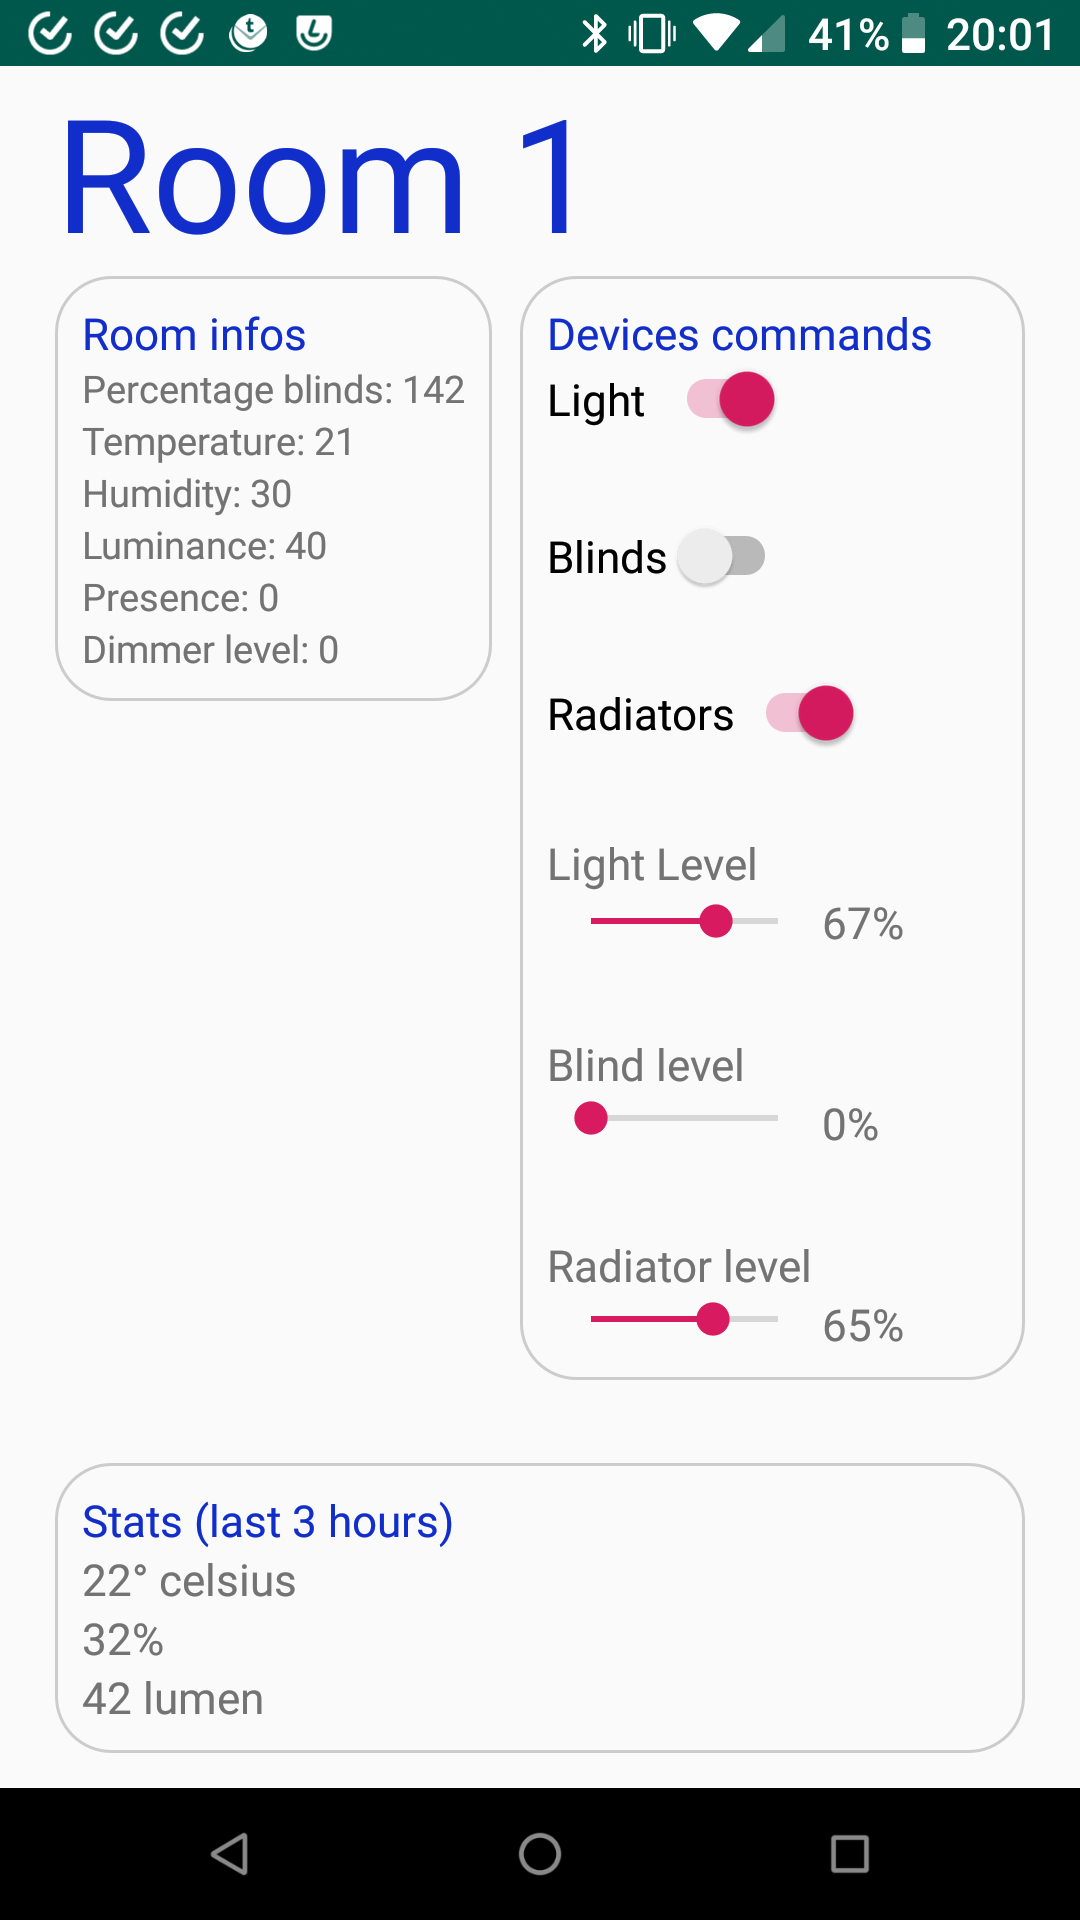
\includegraphics[width=0.5\textwidth]{img/app.png}
    \end{center}
    \caption{Application Android}
    \label{app_android}
\end{figure}

\subsection{Broker Kafka}
Le broker Kafka joue le rôle de coordinateur entre tous les différents clients qui consomment et produisent des messages dans les différents topics. Nous avons choisi de déployer ce broker Kafka sur une instance AWS \cite{aws} avec Docker \cite{docker} et docker-compose \cite{docker-compose}, le rendant accessible par toutes les entités du système.
Nous avons également associé un nom de domaine à cette instance, ce qui permet de la référencer de manière plus lisible et agréable par les clients. Nous avons fait usage des images docker de Confluent \cite{confluent} pour Kafka \cite{cp-kafka} et son Zookeeper \cite{cp-zookeeper}. Elles intègrent un broker Kafka configurable. Le listing \ref{compose-kafka} montre un exemple d'utilisation de ces images dans un \mintinline{text}{docker-compose.yml}. Dans cet exemple, le broker Kafka utilisé est disponible avec l'\acrshort{uri} \mintinline{text}{iot.liatti.ch} sur le port 29092.
\begin{code}
    \begin{minted}[bgcolor=mygray,breaklines,breaksymbol=,linenos,frame=single,stepnumber=1,tabsize=2]{yaml}
version: '3'
services:
  zookeeper:
    image: confluentinc/cp-zookeeper:latest
    environment:
      ZOOKEEPER_CLIENT_PORT: 2181
      ZOOKEEPER_TICK_TIME: 2000
  kafka:
    image: confluentinc/cp-kafka:latest
    depends_on:
      - zookeeper
    ports:
      - 29092:29092
    environment:
      KAFKA_BROKER_ID: 1
      KAFKA_ZOOKEEPER_CONNECT: zookeeper:2181
      KAFKA_ADVERTISED_LISTENERS: PLAINTEXT://kafka:9092,PLAINTEXT_HOST://iot.liatti.ch:29092
      KAFKA_LISTENER_SECURITY_PROTOCOL_MAP: PLAINTEXT:PLAINTEXT,PLAINTEXT_HOST:PLAINTEXT
      KAFKA_INTER_BROKER_LISTENER_NAME: PLAINTEXT
      KAFKA_OFFSETS_TOPIC_REPLICATION_FACTOR: 1
    \end{minted}
    \caption{Utilisation des images Docker de Confluent pour Kafka}
    \label{compose-kafka}
\end{code}

\subsection{\acrshort{rest} server Flask}
Etant donné qu'il n'existe pas encore de librairie permettant d'utiliser directement le client Kafka sur Android, nous avons du mettre en place un adapteur entre Kafka et Android.
Pour ce faire, nous avons utilisé la librairie Flask \cite{flask} de Python 3 qui permet de mettre en place une \acrshort{api} \acrshort{rest}. Ce serveur est connecté à la base de données et au broker Kafka. Le producteur Kafka se charge de transformer les actions reçues sous forme de requêtes HTTP en messages Kafka envoyés directement dans le bon topic, ce qui permet d'effectuer les actions demandées en conséquence (ouverture des stores par exemple). Pour récupérer l'état actuel des \textit{\textit{devices}} ou de la pièce, les derniers logs sont récupérés avec des requêtes à la base de données. Le serveur est déployé dans un container Docker avec docker-compose.

\subsubsection{Routes exposées}
Voici la liste exhaustive des différentes routes mise à disposition par notre \acrshort{api} \acrshort{rest} : 

\paragraph{KNX}

\begin{itemize}
  \item \mintinline{python}{Endpoint: "/open_blinds" -  Method: GET}
  \begin{itemize} 
    \item Params :
    \begin{itemize}
      \item uuid: string
      \item major: int
      \item minor: int
    \end{itemize}

    \item Response : 
    \begin{itemize}
      \item OK: \mintinline{json}{{ "success": true }}
      \item Error: \mintinline{json}{{ "success": false }}
    \end{itemize}
  \end{itemize}
\end{itemize}


\begin{itemize}
  \item \mintinline{python}{Endpoint: "/close_blinds" -  Method: GET}
  \begin{itemize} 
    \item Params :
    \begin{itemize}
      \item uuid: string
      \item major: int
      \item minor: int
    \end{itemize}

    \item Response : 
    \begin{itemize}
      \item OK: \mintinline{json}{{ "success": true }}
      \item Error: \mintinline{json}{{ "success": false }}
    \end{itemize}
  \end{itemize}
\end{itemize}

\begin{itemize}
  \item \mintinline{python}{Endpoint: "/percentage_blinds" -  Method: GET}
  \begin{itemize} 
    \item Params :
    \begin{itemize}
      \item uuid: string
      \item major: int
      \item minor: int
      \item percentage: int
    \end{itemize}

    \item Response : 
    \begin{itemize}
      \item OK: \mintinline{json}{{ "success": true }}
      \item Error: \mintinline{json}{{ "success": false }}
    \end{itemize}
  \end{itemize}
\end{itemize}

\begin{itemize}
  \item \mintinline{python}{Endpoint: "/percentage_radiator" -  Method: GET}
  \begin{itemize} 
    \item Params :
    \begin{itemize}
      \item uuid: string
      \item major: int
      \item minor: int
      \item percentage: int
    \end{itemize}

    \item Response : 
    \begin{itemize}
      \item OK: \mintinline{json}{{ "success": true }}
      \item Error: \mintinline{json}{{ "success": false }}
    \end{itemize}
  \end{itemize}
\end{itemize}


\paragraph{Infos}

\begin{itemize}
  \item \mintinline{python}{Endpoint: "/read_percentage_blinds" -  Method: GET}
  \begin{itemize} 
    \item Params :
    \begin{itemize}
      \item uuid: string
      \item major: int
      \item minor: int
    \end{itemize}

    \item Response : 
    \begin{itemize}
      \item OK: \mintinline{json}{{ "success": true, "percentage": 42 }}
      \item Error: \mintinline{json}{{ "success": false }}
    \end{itemize}
  \end{itemize}
\end{itemize}



\paragraph{OpenZWave}

\begin{itemize}
  \item \mintinline{python}{Endpoint: "/percentage_dimmers" -  Method: GET}
  \begin{itemize} 
    \item Params :
    \begin{itemize}
      \item uuid: string
      \item major: int
      \item minor: int
      \item percentage: int
    \end{itemize}

    \item Response : 
    \begin{itemize}
      \item OK: \mintinline{json}{{ "success": true }}
      \item Error: \mintinline{json}{{ "success": false }}
    \end{itemize}
  \end{itemize}
\end{itemize}

\paragraph{Infos}

\begin{itemize}
  \item \mintinline{python}{Endpoint: "/sensor_get_temperature" -  Method: GET}
  \begin{itemize} 
    \item Params :
    \begin{itemize}
      \item uuid: string
      \item major: int
      \item minor: int
    \end{itemize}

    \item Response : 
    \begin{itemize}
      \item OK: \mintinline{json}{{ "success": true, "value": 23 }}
      \item Error: \mintinline{json}{{ "success": false }}
    \end{itemize}
  \end{itemize}
\end{itemize}

\begin{itemize}
  \item \mintinline{python}{Endpoint: "/sensor_get_humidity" -  Method: GET}
  \begin{itemize} 
    \item Params :
    \begin{itemize}
      \item uuid: string
      \item major: int
      \item minor: int
    \end{itemize}

    \item Response : 
    \begin{itemize}
      \item OK: \mintinline{json}{{ "success": true, "value": 23 }}
      \item Error: \mintinline{json}{{ "success": false }}
    \end{itemize}
  \end{itemize}
\end{itemize}

\begin{itemize}
  \item \mintinline{python}{Endpoint: "/sensor_get_luminance" -  Method: GET}
  \begin{itemize} 
    \item Params :
    \begin{itemize}
      \item uuid: string
      \item major: int
      \item minor: int
    \end{itemize}

    \item Response : 
    \begin{itemize}
      \item OK: \mintinline{json}{{ "success": true, "value": 23 }}
      \item Error: \mintinline{json}{{ "success": false }}
    \end{itemize}
  \end{itemize}
\end{itemize}

\begin{itemize}
  \item \mintinline{python}{Endpoint: "/sensor_get_motion" -  Method: GET}
  \begin{itemize} 
    \item Params :
    \begin{itemize}
      \item uuid: string
      \item major: int
      \item minor: int
    \end{itemize}

    \item Response : 
    \begin{itemize}
      \item OK: \mintinline{json}{{ "success": true, "value": 23 }}
      \item Error: \mintinline{json}{{ "success": false }}
    \end{itemize}
  \end{itemize}
\end{itemize}

\begin{itemize}
  \item \mintinline{python}{Endpoint: "/dimmer_get_level" -  Method: GET}
  \begin{itemize} 
    \item Params :
    \begin{itemize}
      \item uuid: string
      \item major: int
      \item minor: int
    \end{itemize}

    \item Response : 
    \begin{itemize}
      \item OK: \mintinline{json}{{ "success": true, "value": 23 }}
      \item Error: \mintinline{json}{{ "success": false }}
    \end{itemize}
  \end{itemize}
\end{itemize}

\paragraph{Autres routes}

\begin{itemize}
  \item \mintinline{python}{Endpoint: "/get_beacons" -  Method: GET}
  \begin{itemize}
    \item Response : 
    \begin{itemize}
      \item OK: \mintinline{json}{{ "success": true, "beacons": 23 }}
      \item Error: \mintinline{json}{{ "success": false }}
    \end{itemize}
  \end{itemize}
\end{itemize}

\begin{itemize}
  \item \mintinline{python}{Endpoint: "/get_devices" -  Method: GET}
  \begin{itemize} 
    \item Params :
    \begin{itemize}
      \item uuid: string
      \item major: int
      \item minor: int
    \end{itemize}

    \item Response : 
    \begin{itemize}
      \item OK: \mintinline{json}{{ "success": true, "devices": 23 }}
      \item Error: \mintinline{json}{{ "success": false }}
    \end{itemize}
  \end{itemize}
\end{itemize}

\paragraph{Stats}

\begin{itemize}
  \item \mintinline{python}{Endpoint: "/avg_temperature" -  Method: GET}
  \begin{itemize} 
    \item Params :
    \begin{itemize}
      \item uuid: string
      \item major: int
      \item minor: int
    \end{itemize}

    \item Response : 
    \begin{itemize}
      \item OK: \mintinline{json}{{ "success": true, "avg_temperature": 23 }}
      \item Error: \mintinline{json}{{ "success": false }}
    \end{itemize}
  \end{itemize}
\end{itemize}

\begin{itemize}
  \item \mintinline{python}{Endpoint: "/avg_humidity" -  Method: GET}
  \begin{itemize} 
    \item Params :
    \begin{itemize}
      \item uuid: string
      \item major: int
      \item minor: int
    \end{itemize}

    \item Response : 
    \begin{itemize}
      \item OK: \mintinline{json}{{ "success": true, "avg_humidity": 23 }}
      \item Error: \mintinline{json}{{ "success": false }}
    \end{itemize}
  \end{itemize}
\end{itemize}

\begin{itemize}
  \item \mintinline{python}{Endpoint: "/avg_luminance" -  Method: GET}
  \begin{itemize} 
    \item Params :
    \begin{itemize}
      \item uuid: string
      \item major: int
      \item minor: int
    \end{itemize}

    \item Response : 
    \begin{itemize}
      \item OK: \mintinline{json}{{ "success": true, "avg_luminance": 23 }}
      \item Error: \mintinline{json}{{ "success": false }}
    \end{itemize}
  \end{itemize}
\end{itemize}




\subsection{Modules KNX et Openzwave}
En se basant sur le code des exercices KNX et Openzwave réalisés en cours, nous avons créé deux modules reliant d'une part Kafka et KNX et d'autre part Kafka et Openzwave. Ces deux modules ont un fonctionnement similaire, ils sont constitués d'une librairie reprenant les méthodes pour communiquer avec KNX ou Openzwave et exposant les différentes méthodes relatives à l'utilisation des \textit{\textit{devices}}. Ils sont également constitués d'un fichier principal (\mintinline{text}{knx.py} et \mintinline{text}{zwave.py}), chaque fichier démarre un thread producteur Kafka, envoyant à intervalles réguliers les valeurs des stores, des senseurs et \textit{dimmers} Openzwave, et un thread consommateur Kafka, écoutant sur le topic "knx" ou "zwave" les commandes à effectuer sur les \textit{\textit{devices}}.

\subsection{Protocole des messages}
En ce qui concerne les messages consommés par KNX et Openzwave, nous avons choisi de définir notre propre protocole.
Celui-ci fait correspondre la clé du message reçu à l'action à effectuer et le contenu du message aux éventuels paramètres à transmettre. Ces différents paramètres sont au format \acrshort{json} puis encodés en bytes afin d'être transmis au broker Kafka et consommés par une autre entité.

\subsubsection{KNX}
Pour KNX nous retrouvons les messages suivants : 
\paragraph{Production}
\begin{itemize}
    \item \mintinline{text}{read_percentage_blinds} : Ce messages est produit à intervalles de 5 secondes, il permet d'envoyer dans le topic \mintinline{text}{knx} le pourcentage d'ouverture de tous les stores de toutes les salles. 
\end{itemize}

\paragraph{Consommation}
L'étage et la chambre permettent d'identifier l'appareil sur lequel il faut agir, pour cela ces deux paramètres sont donnés dans le corps du message ce qui permet d'intéragir avec le bon \textit{device} en fonction de la position de l'utilisateur.
\begin{itemize}
    \item \mintinline{text}{open_blinds} : permet d'ouvrir les stores (100\%)
    \item \mintinline{text}{close_blinds} : permet de fermer les stores (0\%)
    \item \mintinline{text}{percentage_blinds} : met les stores à un certain pourcentage qui est passé dans la valeur du message
    \item \mintinline{text}{percentage_radiator} : met les radiateurs à un certain pourcentage qui est passé dans la valeur du message
\end{itemize}

\subsubsection{Openzwave}
Openzwave est capable de traiter les messages suivants : 
\paragraph{Production}
\begin{itemize}
    \item \mintinline{text}{sensors_get_temperature} : produit la valeur de température de chaque senseur
    \item \mintinline{text}{sensors_get_humidity} : produit la valeur de l'humidité de chaque senseur
    \item \mintinline{text}{sensors_get_luminance} : produit la valeur de la luminance de chaque senseur
    \item \mintinline{text}{sensors_get_motion} : produit une indication de présence de chaque senseur
    \item \mintinline{text}{dimmers_get_level} : produit la valeur de chaque variateur (\textit{dimmer})
\end{itemize}

\paragraph{Consommation}
\begin{itemize}
    \item \mintinline{text}{dimmers_set_level} : met les \textit{dimmers} à un certain pourcentage
\end{itemize}

\subsection{Base de données}
En ce qui concerne la base de données, nous avons opté pour une base relationnelle avec MySQL \cite{mysql} qui nous a permis de représenter les différentes entités et les lier facilement et de manière efficace. Comme représenté sur la figure \ref{db_schema}, la base comporte six tables :
\begin{itemize}
    \item \mintinline{text}{Beacon} : contient tous les Beacons et dans quelle pièce
    \item \mintinline{text}{Room} : contient les différentes pièces et à quel étage
    \item \mintinline{text}{Device} : contient tous les \textit{devices} (KNX et Openzwave), identifiés de manière unique et dans quelle pièce ils se trouvent
    \item \mintinline{text}{KnxNode} : contient les informations concernant les \textit{devices} KNX uniquement (type, bloc et étage)
    \item \mintinline{text}{ZwaveNode} : contient les informations concernant les \textit{devices} Openzwave uniquement (identifiant dans le réseau Openzwave et nom)
    \item \mintinline{text}{Log} : contient les logs produits par tous les \textit{devices} avec la valeur, le type de valeur et le \textit{timestamp} (à la seconde) de la mesure
\end{itemize}
Ces relations permettent des usages tels que :
\begin{itemize}
    \item Pour un Beacon donné, retrouver tous les logs des \textit{devices} de la pièce associée
    \item Avec un type, bloc et étage KNX donnés, retrouver dans quelle pièce ils se trouvent
    \item Réaliser des statistiques sur les logs, comme la température moyenne dans une pièce
\end{itemize}

Voici le diagramme représentant notre base de données :
\begin{figure}
    \begin{center}
        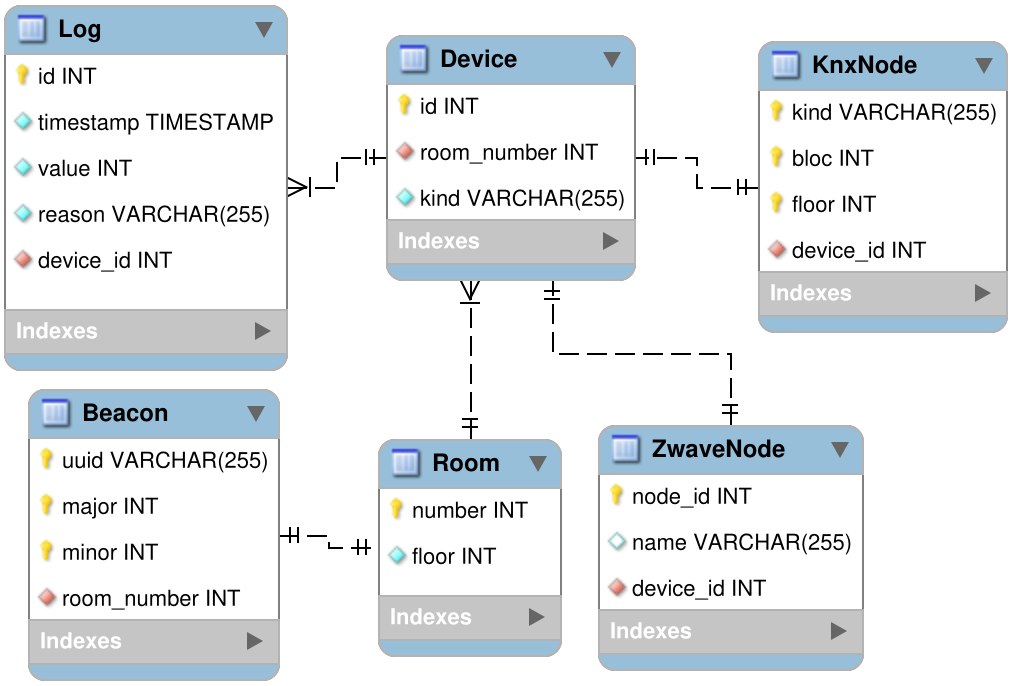
\includegraphics[width=0.8\textwidth]{img/mysql-shema.png}
    \end{center}
    \caption{Schéma relationnel de la base de données}
    \label{db_schema}
\end{figure}

\subsection{Automatic controller}
Le controleur automatique est déployé dans un container Docker avec docker-compose. Son rôle est de gérer les états des devices dans les différentes salles. Pour ce faire, il lit les messages dans les topics Kafka propres à KNX et Openzwave. En fonction des informations récuprées sur les devices, il applique certaines règlès logiques afin de contrôler les devices automatiquement.
Les différentes règles sont les suivants : (A savoir que les différentes valeurs définies sont arbitraires et modifiable très facilement)
\begin{itemize}
  \item Si aucune présence est detectée dans la pièce, le radiateur se met automatiquement à 10\% afin d'économiser de l'énergie
  \item Si quelqu'un est dans la pièce, le radiateur se règle à 90\% afin qu'il n'ai pas froid
  \item Si l'humidité est supérieure à 50\% les stores de la pièce se ferment
  \item Si il est plus tôt que 19 heure, que quelqu'un est présent dans la pièce et que la lumonosité est faible, les stores s'ouvrent automatiquement
  \item Si l'heure actuelle est comprise entre 19 heure et 7 heure du matin et que quelqu'un est présent dans la pièce, ou, si la luminosité est trop faible, la lumière s'allume alors automatiquement. Dans un des cas contraires, la lumière s'éteint.
\end{itemize}
L'Automatic controller est déployé dans un container Docker avec docker-compose.

\subsection{DB to Kafka}
Pour minimiser les dépendances à la base de données pour les modules KNX, OpenZWave et Automatic controller, nous avons réalisé un connecteur, \mintinline{python}{db_to_kafka.py}, qui produit dans le topic Kafka \mintinline{text}{db} la liste de tous les \textit{devices} avec leur type effectif (KNX ou OpenZWave) et leur emplacement physique (dans quelle pièce ils se trouvent). Ainsi, les modules reliés à Kafka nécessitant les informations sur les \textit{devices} peuvent relire le topic \mintinline{text}{db} à partir de l'\textit{offset} zéro pour obtenir tous les \textit{devices}. Ce module est déployé dans un container Docker avec docker-compose.

\subsection{Logs et statistiques}
Pour garder une trace des valeurs des différents \textit{devices}, un module \mintinline{python}{logs.py} écoute et consomme les messages Kafka des topics \mintinline{text}{knx} et \mintinline{text}{zwave} concernant la lecture des valeurs et réalise des insertions en base de données dans la table \mintinline{text}{Log}. Il est donc aisé de retrouver les anciennes valeurs des capteurs et réaliser des statistiques avec. Ce module est déployé dans un container Docker avec docker-compose.
